\documentclass[a4paper]{article}
\usepackage[paper=A4,pagesize]{typearea}
\usepackage[right=2.5cm,left=3cm,top=2.5cm,bottom=2.5cm,headsep=0.75cm,footskip=1cm]{geometry}%%Bordes
\usepackage[utf8]{inputenc}%%Acentos
\usepackage[spanish]{babel}%%
\usepackage{graphicx}%% tablas e imagenes
\usepackage{hyperref}%% urls
\usepackage{caption}
\usepackage{biblatex}
\addbibresource{ref.bib}
\hypersetup{
pdftitle={Manual Symfony},
pdfauthor={krosf},
pdfkeywords={PW,Symfony,PHP}
}
\begin{document}

%
% Portada
%

\begin{titlepage}
    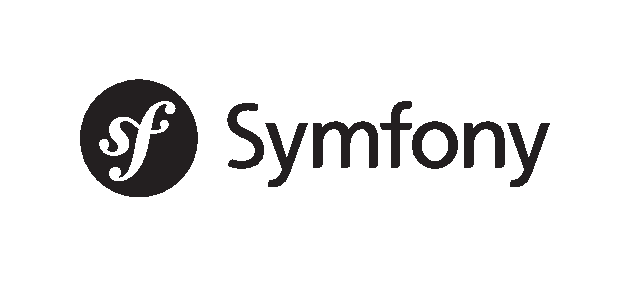
\includegraphics[width=0.5\textwidth]{assets/symfony_logo.eps}
   \begin{center}
       \vspace*{6cm}
 
       \textbf{\LARGE{Tutorial Laravel}}
 
       \vspace{0.5cm}
       \textbf{\LARGE{Carlos Rodrigo Sanabria Flores}}
       \vspace{2cm}
       \vfill
       Programación Web\\
       Grado en Ingeniería Informática\\
       Universidad de Cádiz\\
       \today
       \vspace{2cm}
 
   \end{center}
\end{titlepage}
\clearpage
\setcounter{page}{1}

%
% Indice
%
\tableofcontents
\listoffigures
\newpage

%
% Caracteristicas
%
\section{Características de Symfony}

Symfony se diseñó para que se ajustara a los siguientes requisitos:

\begin{itemize}
    \item Fácil de instalar y configurar en la mayoría de plataformas.
    \item Independiente del sistema gestor de bases de datos.
    \item Sencillo de usar en la mayoría de casos, pero lo suficientemente flexible como para adaptarse a los casos más complejos.
    \item Basado en la premisa de "convenir en vez de configurar", en la que el desarrollador solo debe configurar aquello que no es convencional.
    \item Sigue la mayoría de mejores prácticas y patrones de diseño para la web.
    \item Preparado para aplicaciones empresariales y adaptable a las políticas y arquitecturas propias de cada empresa, además de ser lo suficientemente estable como para desarrollar aplicaciones a largo plazo.
    \item Código fácil de leer que incluye comentarios de phpDocumentor y que permite un mantenimiento muy sencillo.
    \item Fácil de extender, lo que permite su integración con librerías desarrolladas por terceros. 
\end{itemize}

%
% Pre-requisitos
%
\section{Pre-requisitos}
El funcionamiento de Symfony requiere de algunos elementos previos de los cuales debemos asegurarnos estén disponibles en nuestro equipo. Sin dichos elementos no podremos poner a utilizar el framework.

\begin{itemize}
    \item PHP 7.2.5 o superior y las siguientes extensiones de php (generalmente activas por defecto): \href{https://www.php.net/book.ctype}{Ctype}, \href{https://www.php.net/book.iconv}{iconv}, \href{https://www.php.net/book.json}{JSON}, \href{https://www.php.net/book.pcre}{PCRE}, \href{https://www.php.net/book.session}{Session}, \href{https://www.php.net/book.simplexml}{SimpleXML}, y \href{https://www.php.net/book.tokenizer}{Tokenizer}; 
    \item \href{https://getcomposer.org/download/}{Composer}
\end{itemize}

Opcionalmente podemos instalar la aplicación \href{https://symfony.com/download}{Symfony CLI}. 
Esto crea un binario llamado Symfony que proporciona todas las herramientas que necesitas para desarrollar y ejecutar una aplicación Symfony localmente.


%
% Crear un proyecto
%

\section{Creando una Aplicación de Symfony}
\subsection{Symfony CLI}
\begin{figure}[ht]
    \centering
    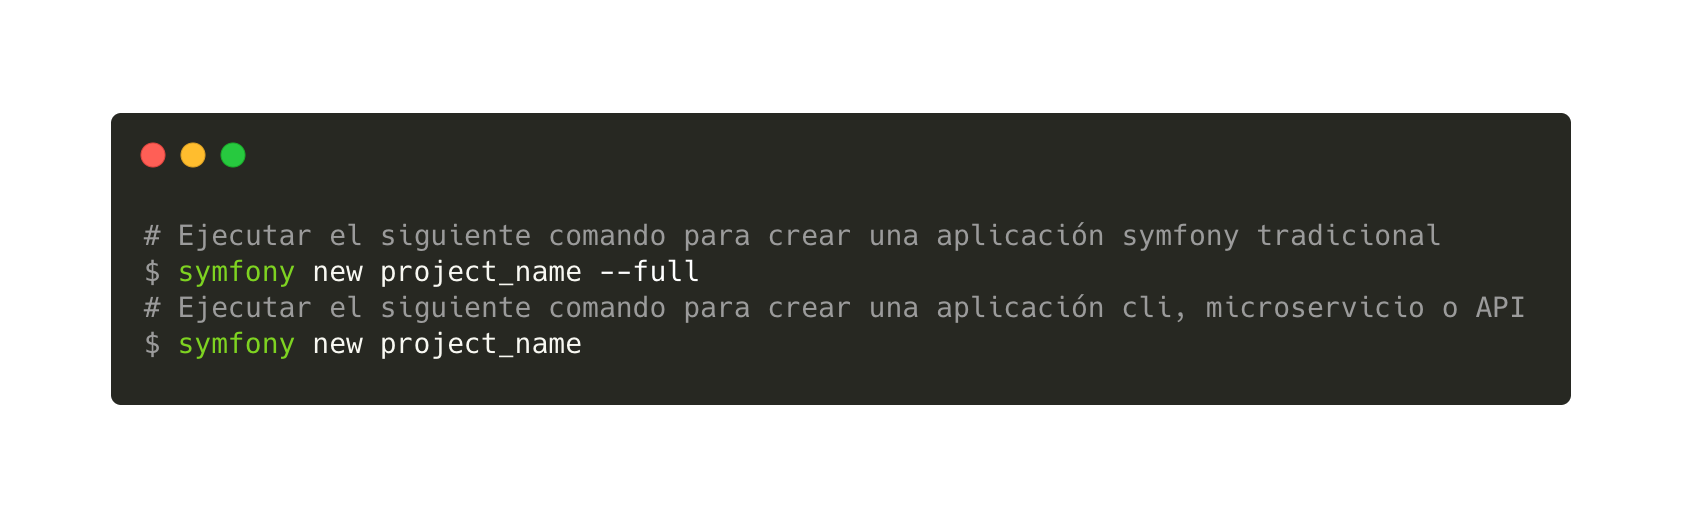
\includegraphics[width=\textwidth]{../assets/symfony_new.png}
    \caption{Nuevo proyecto symfony con el cli}
    \label{fig:symfony_new}
\end{figure}
\clearpage
\subsection{Composer}

\begin{figure}[ht]
    \centering
    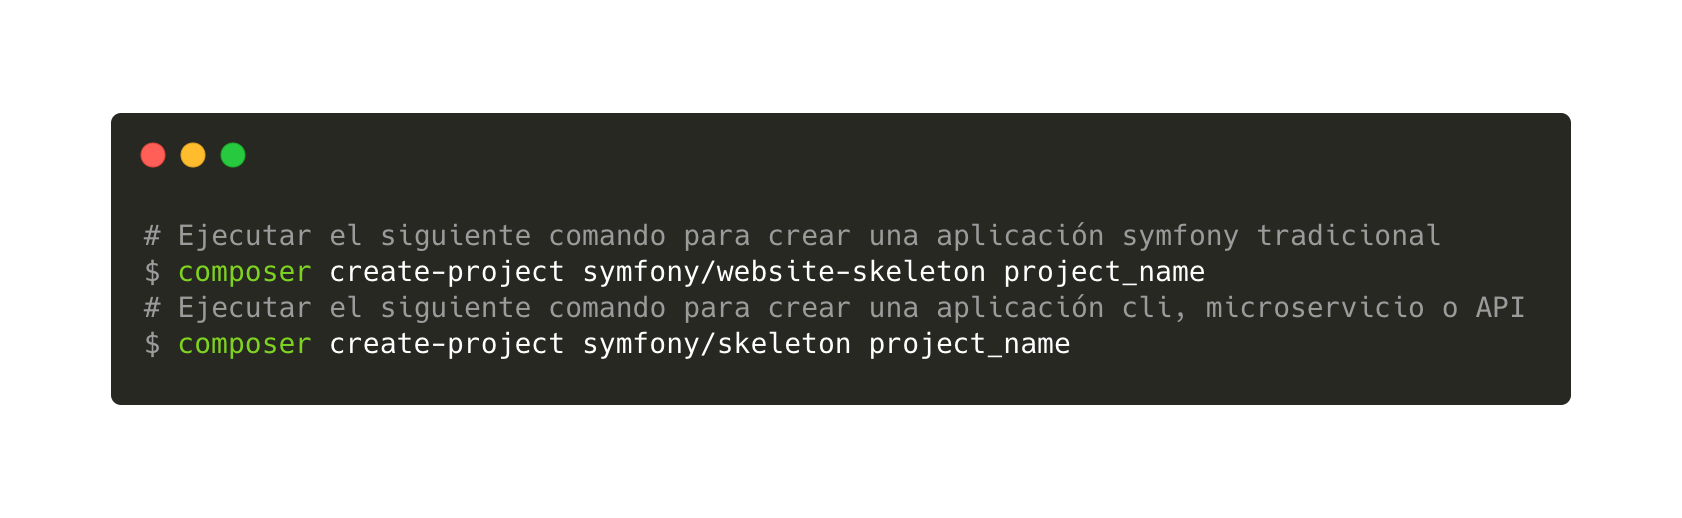
\includegraphics[width=\textwidth]{../assets/composer_create.png}
    \caption{Nuevo proyecto symfony con composer}
    \label{fig:composer_create}
\end{figure}

%
% Patron MVC
%
\section{El Patrón MVC}
Symfony está basado en un patrón clásico del diseño web conocido como arquitectura MVC, que está formado por tres niveles:
\begin{itemize}
    \item El Modelo representa la información con la que trabaja la aplicación, es decir, su lógica de negocio.
    \begin{itemize}
        \item Se encarga de la abstracción de la lógica relacionada con los datos, haciendo que la vista y las acciones sean independientes de, por ejemplo, el tipo de gestor de bases de datos utilizado por la aplicación.
    \end{itemize}
    \item La Vista transforma el modelo en una página web que permite al usuario interactuar con ella.
    \item El Controlador se encarga de procesar las interacciones del usuario y realiza los cambios apropiados en el modelo o en la vista.
    \begin{itemize}
        \item También se encarga de aislar al modelo y a la vista de los detalles del protocolo utilizado para las peticiones (HTTP, consola de comandos, email, etc.).
    \end{itemize}
\end{itemize}
\subsection{Separación en capas más allá del MVC}
El principio más importante de la arquitectura MVC es la separación del código del programa en tres capas, dependiendo de su naturaleza. La lógica relacionada con los datos se incluye en el modelo, el código de la presentación en la vista y la lógica de la aplicación en el controlador. 

La programación se puede simplificar si se utilizan otros patrones de diseño. De esta forma, las capas del modelo, la vista y el controlador se pueden subdividir en más capas. 

\subsection{Orientación a objetos}
La orientación a objetos permite a los desarrolladores trabajar con objetos de la vista, objetos del controlador y clases del modelo, transformando las funciones de los ejemplos anteriores en métodos. \textbf{Se trata de un requisito obligatorio para las arquitecturas de tipo MVC}.

\subsection{La implementación del MVC que realiza Symfony}
Piensa por un momento cuántos componentes se necesitan para realizar una página sencilla que muestre un listado de las entradas o artículos de un blog, son necesarios los siguientes componentes:
\begin{itemize}
    \item La capa del Modelo
    \begin{itemize}
        \item Abstracción de la base de datos
        \item Acceso a los datos
    \end{itemize}
    \item La capa de la Vista
    \begin{itemize}
        \item Vista
        \item Plantilla
        \item Layout
    \end{itemize}
    \item La capa del Controlador
    \begin{itemize}
        \item Controlador frontal
        \item Acción
    \end{itemize}
\end{itemize}

En total son siete scripts, lo que parecen muchos archivos para abrir y modificar cada vez que se crea una página. Afortunadamente, Symfony simplifica este proceso.\\
Symfony toma lo mejor de la arquitectura MVC y la implementa de forma que el desarrollo de aplicaciones sea rápido y sencillo.\\

En primer lugar, el controlador frontal y el layout son comunes para todas las acciones de la aplicación. Se pueden tener varios controladores y varios layouts, pero solamente es obligatorio tener uno de cada. El controlador frontal es un componente que sólo tiene código relativo al MVC, por lo que no es necesario crear uno, ya que Symfony lo genera de forma automática.\\

La otra buena noticia es que las clases de la capa del modelo también se generan automáticamente, en función de la estructura de datos de la aplicación.\\

El ORM se encarga de crear el esqueleto o estructura básica de las clases y genera automáticamente todo el código necesario. Cuando el ORM encuentra restricciones de claves foráneas (o externas) o cuando encuentra datos de tipo fecha, crea métodos especiales para acceder y modificar esos datos, por lo que la manipulación de datos se convierte en un juego de niños.\\

La abstracción de la base de datos es completamente transparente para el programador, ya que se realiza de forma nativa mediante PDO PHP Data Objects). Así, si se cambia el sistema gestor de bases de datos en cualquier momento, no se debe reescribir ni una línea de código, ya que tan sólo es necesario modificar un parámetro en un archivo de configuración. 
Por último, la lógica de la vista se puede transformar en un archivo de configuración sencillo, sin necesidad de programarla.\\
Por si fuera poco, crear la aplicación con Symfony permite crear páginas XHTML válidas, depurar fácilmente las aplicaciones, crear una configuración sencilla, abstracción de la base de datos utilizada, enrutamiento con URL limpias, varios entornos de desarrollo y muchas otras utilidades para el desarrollo de aplicaciones. 
\clearpage

%
% Primera Pagina
%
\section{Primera Pagina en Symfony}
Crear una nueva página, ya sea una página HTML o JSON, es un proceso de dos pasos:
\begin{itemize}
  \item \textbf{Crear una ruta:} Una ruta es la URL (por ejemplo, /about) a su página y apunta a un controlador
  \item \textbf{Crear un controlador}: Un controlador es un script PHP de funciones que se encargará de construir las páginas. Toma la información de respuesta creando un objeto de Symfony de tipo Response, cada uno puede contener contenido HTML, cadenas JSON o incluso archivos binarios, tanto imágenes como PDF.
\end{itemize}
\subsection{Creando una página: Route y Controller}
Supongamos que queremos crear la página - \texttt{/lucky/number} - que genera números de la suerte (de forma aleatoria) y los imprime. Para hacer eso, creamos una “Controller class” que la llamaremos LuckyController y un método “controller” que será ejecutado cada vez que vayamos a \texttt{/lucky/number}:


\begin{figure}[ht]
  \centering
  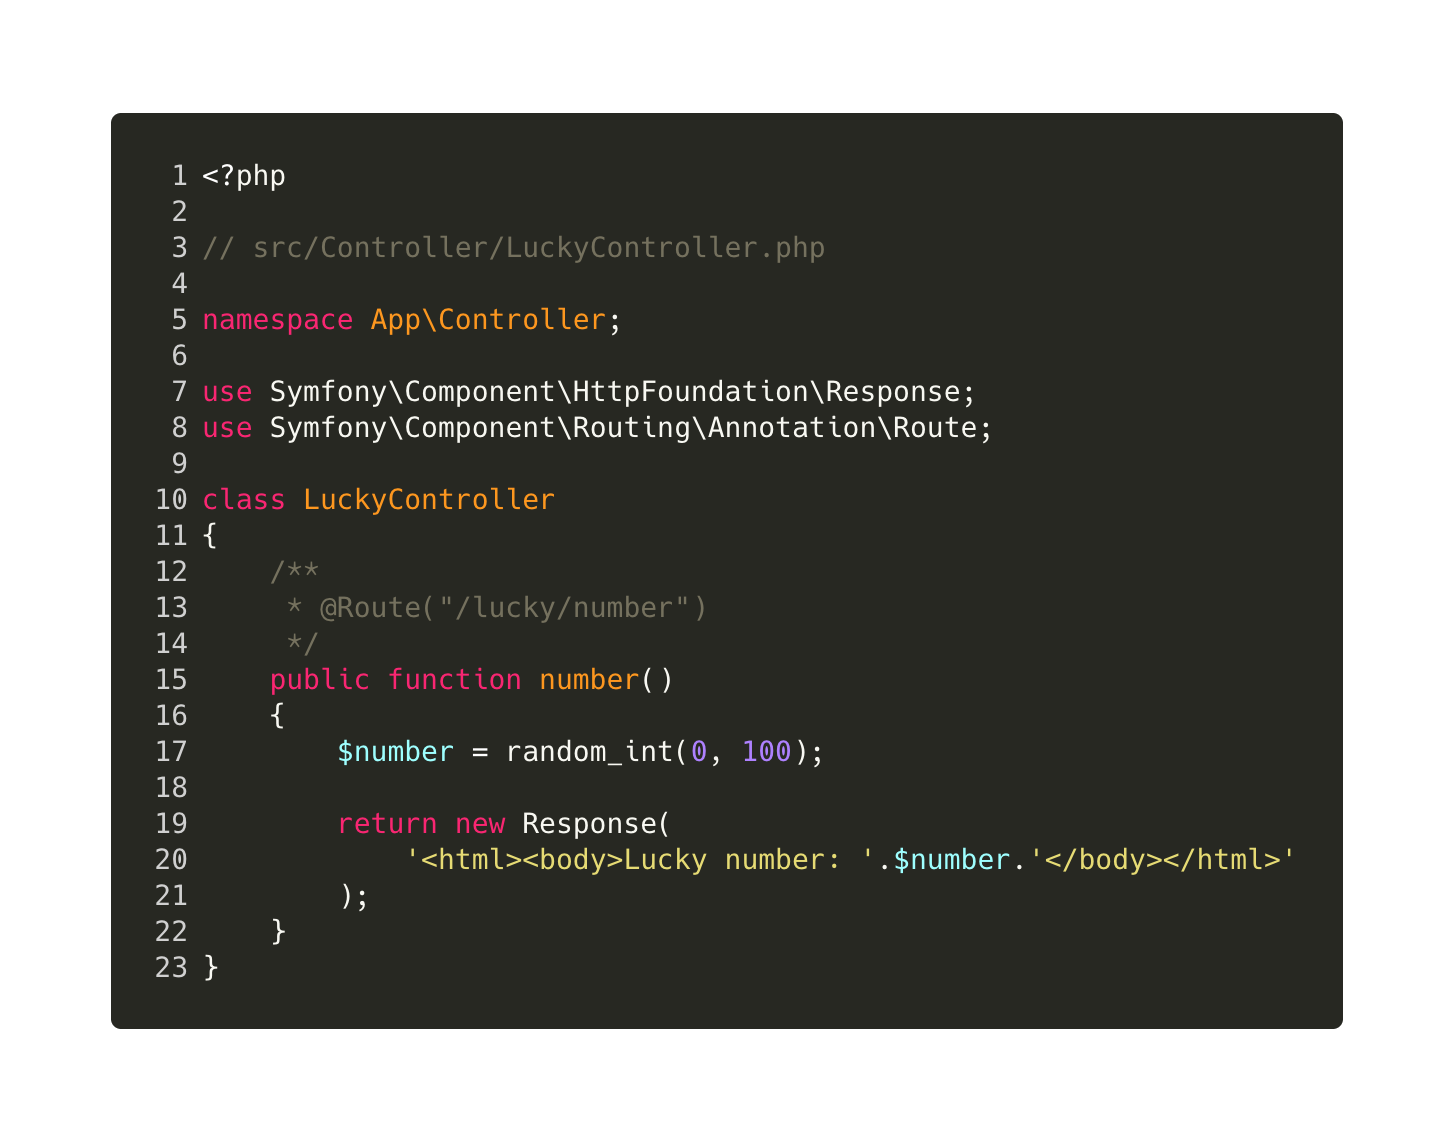
\includegraphics[width=\textwidth]{../assets/lucky_controller.png}
  \caption{Controlador \textbf{/luck/number}}
  \label{fig:lucky_controller}
\end{figure}

Podemos visualizar el resultado en \href{http://localhost:8888/lucky/number}{http://localhost:8888/lucky/number}

\begin{figure}[ht]
  \centering
  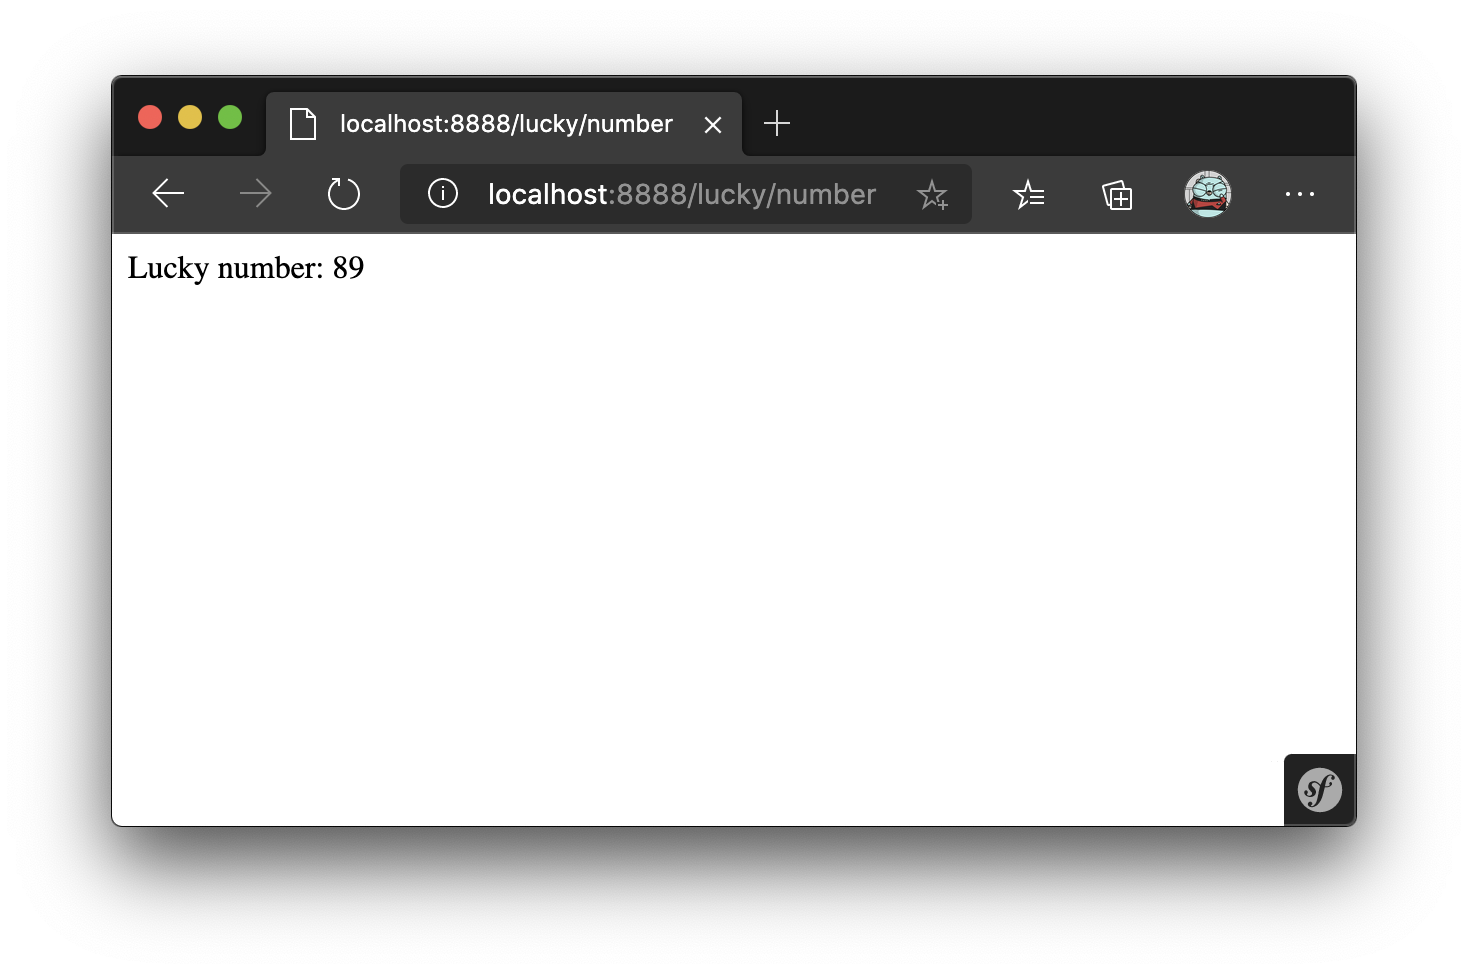
\includegraphics[width=\textwidth]{../assets/lucky_number.png}
  \caption{Respuesta \textbf{/luck/number}}
  \label{fig:lucky_number}
\end{figure}
\clearpage
\subsection{La barra de herramientas de depuración web}
Una de las características principales de Symfony es la Barra de herramientas de depuración web: una barra que muestra una gran cantidad de información de depuración en la parte inferior de la página durante el desarrollo. Todo esto está incluido de por defecti usando un paquete de Symfony llamado \texttt{symfony/profiler-pack}.

\begin{figure}[ht]
  \centering
  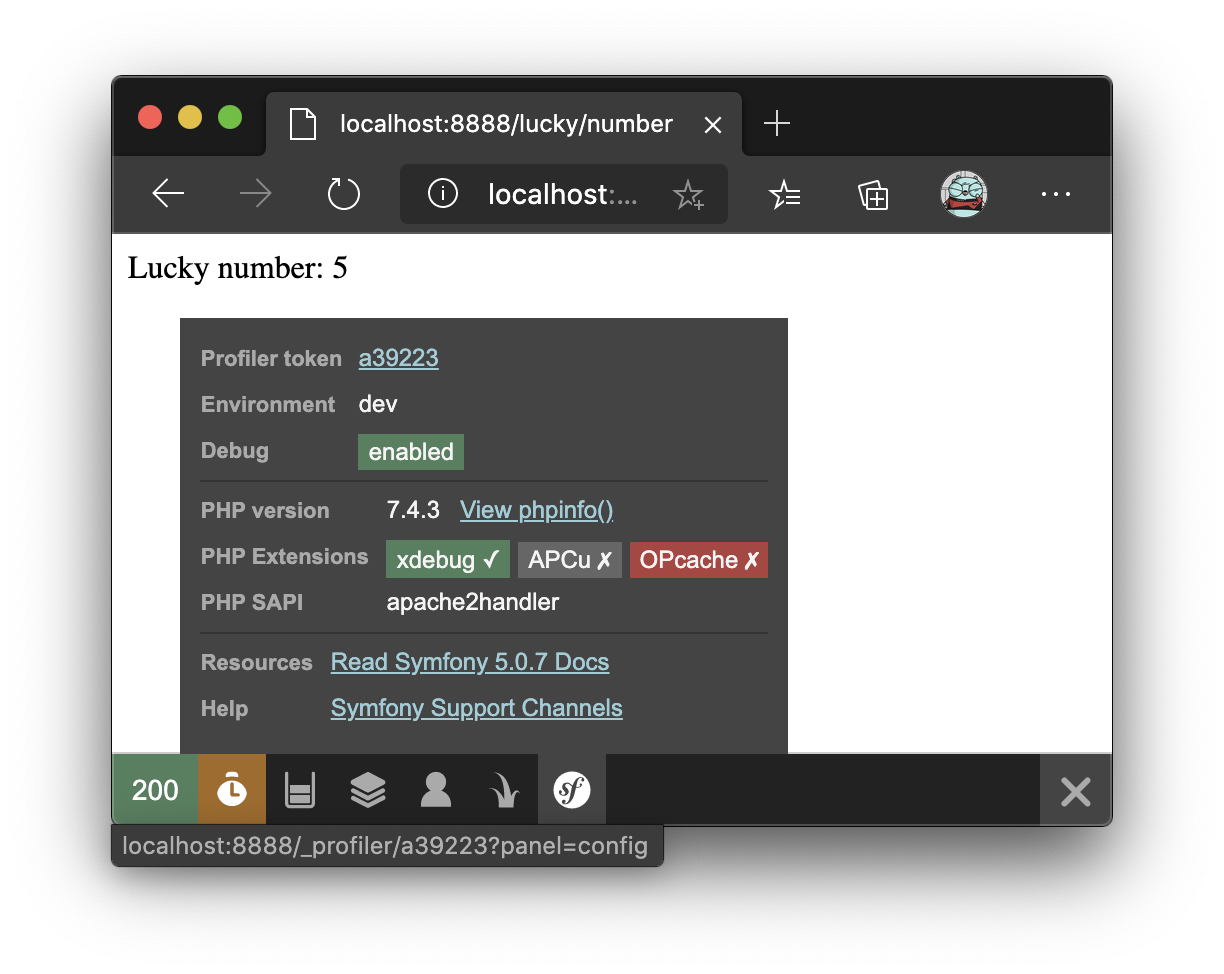
\includegraphics[width=\textwidth]{../assets/symfony_debug_bar.png}
  \caption{Barra de herramientas de depuración}
  \label{fig:symfony_debug_bar}
\end{figure}
\clearpage
\subsection{Renderizando una plantilla}

Si está devolviendo HTML desde su controlador, probablemente quiera renderizar una plantilla. Afortunadamente, Symfony viene con \href{https://twig.symfony.com/}{Twig}: un lenguaje de plantillas que es fácil, poderoso y realmente bastante divertido.
\medskip\\
Asegúrese de que LuckyController extienda la clase abstracta AbstractController de Symfony:

\begin{figure}[ht]
  \centering
  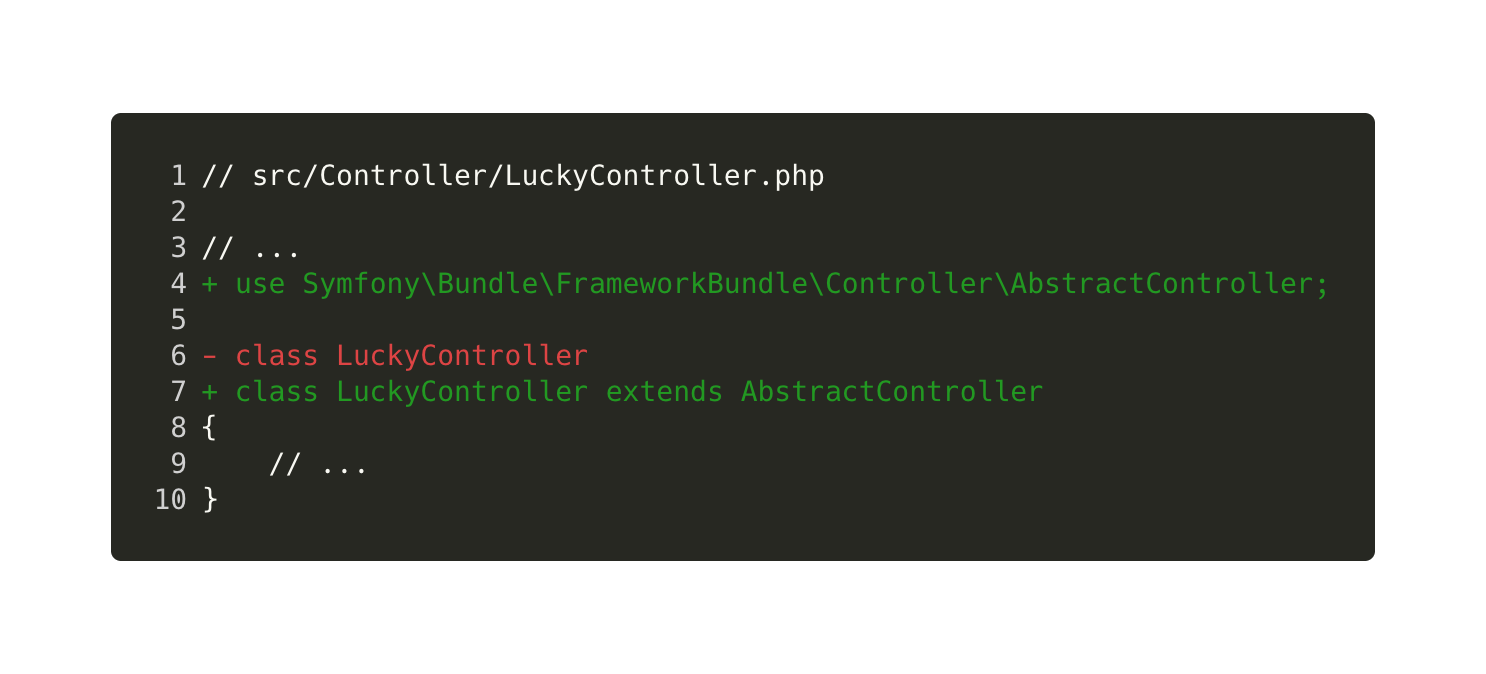
\includegraphics[width=\textwidth]{../assets/diff_lucky_controller.png}
  \caption{Heredar desde AbstractController}
  \label{fig:diff_lucky_controller}
\end{figure}

Ahora, use la práctica función \texttt{render()} para renderizar una plantilla. Pase una variable numérica para que puedas usarlo en Twig:

\begin{figure}[ht]
  \centering
  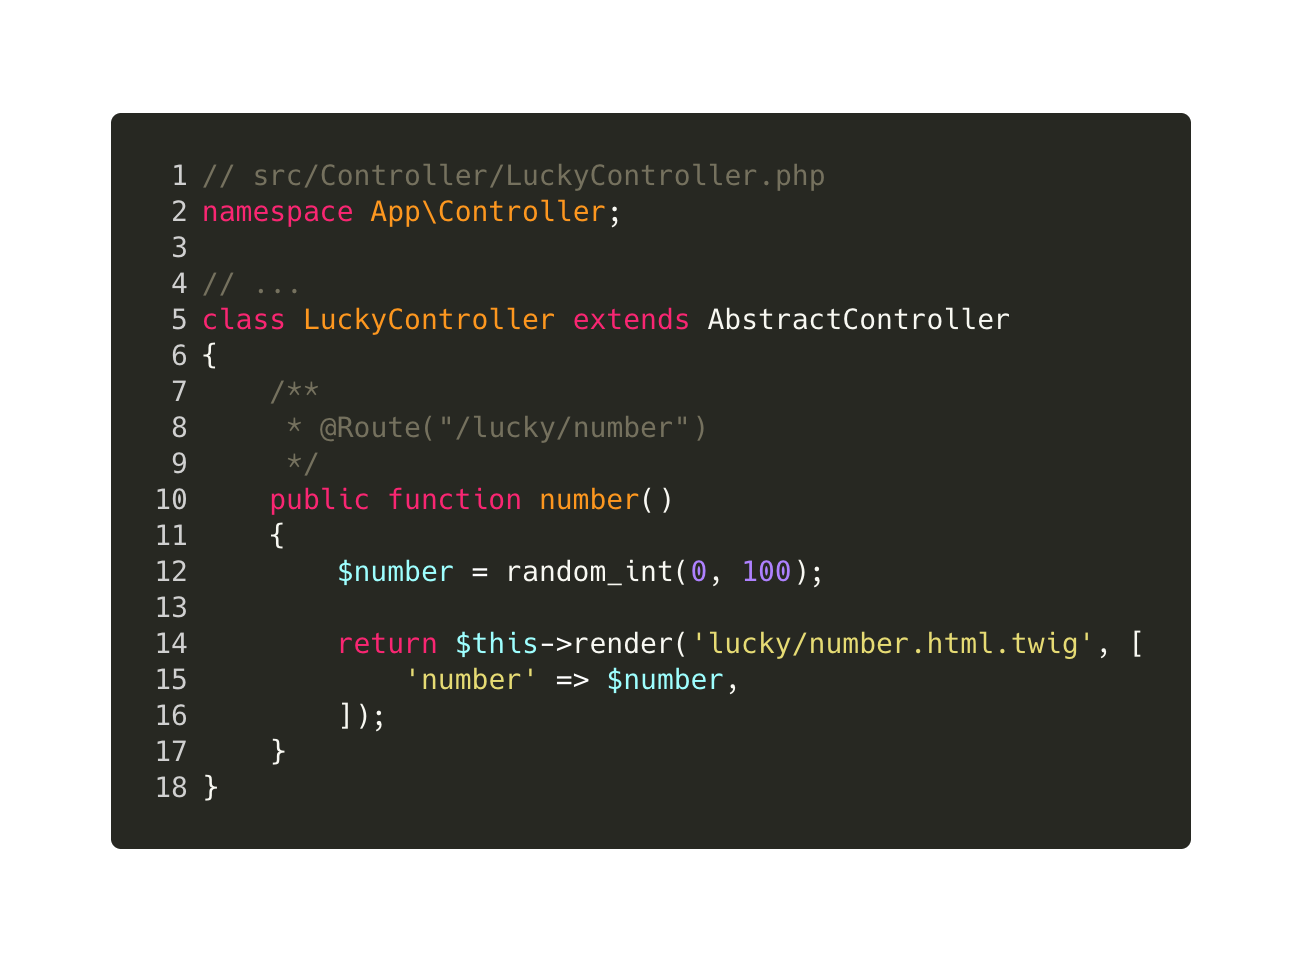
\includegraphics[width=\textwidth]{../assets/lucky_number_twig.png}
  \caption{Uso del metodo \texttt{render()}}
  \label{fig:lucky_number_twig}
\end{figure}
\clearpage
Los archivos de plantilla viven en el directorio \texttt{templates/}, que se creó automáticamente cuando instaló Twig. Cree un nuevo directorio \texttt{templates/lucky} con un nuevo archivo \texttt{number.html.twig} dentro:

\begin{figure}[ht]
  \centering
  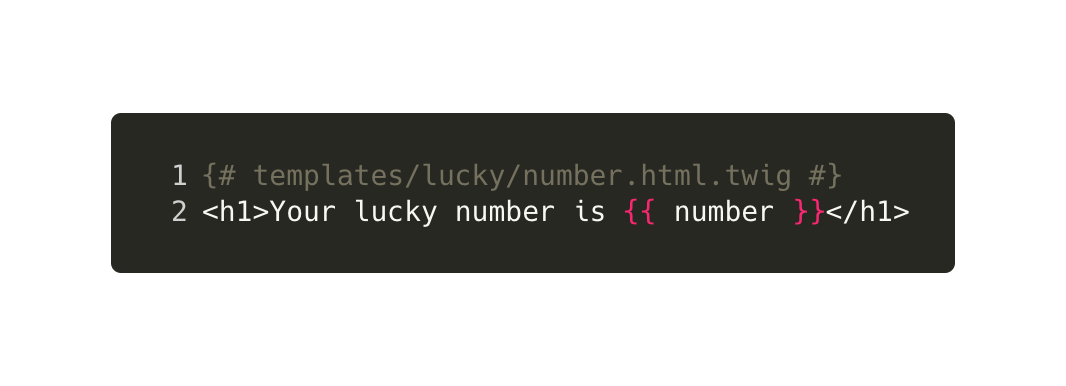
\includegraphics[width=\textwidth]{../assets/lucky_number_template.png}
  \caption{Plantilla \texttt{/lucky/number}}
  \label{fig:lucky_number_template}
\end{figure}

La sintaxis utilizada {{ number }} es para imprimir las variables en el sistema de trabajo de Twig.

\subsection{Estructura del proyecto}
Ya hemos estado trabajando en dos de las carpetas más importantes de nuestro proyecto, ahora veremos la importancia y uso de las demás dentro de la estructura que nos ofrece Symfony:
\begin{itemize}
  \item[\textbf{\texttt{config/}}] Contiene la configuración donse se configurarán rutas, servicios y paquetes.
  \item[\textbf{\texttt{src/}}] El código PHP a utilizar lo colocamos dentro de esta carpeta.
  \item[\textbf{\texttt{templates/}}] Todas las plantillas Twig viven aquí.
  \item[\textbf{\texttt{bin/}}] Aquí vive el famoso archivo \texttt{bin/console} (y otros archivos ejecutables menos importantes).
  \item[\textbf{\texttt{var/}}] Aquí es donde se almacenan los archivos creados automáticamente, como los archivos de caché (\texttt{var/cache/}) y los registros (\texttt{var/log/}).
  \item[\textbf{\texttt{vendor/}}] ¡Aquí viven bibliotecas de terceros! Estos se descargan a través del administrador de paquetes \href{https://getcomposer.org/}{Composer}.
  \item[\textbf{\texttt{public/}}] Carpeta raíz del proyecto, en esta carpeta introduciremos todos los elementos públicos(CSS, JS, imágenes...)
\end{itemize}

La mayoría de las veces, trabajaremos en \texttt{src/}, \texttt{templates/} o \texttt{config/}.
\clearpage

%
% Tutorial
%
\section{Tutorial}
\subsection{Creación del Proyecto}
\begin{figure}[ht]
  \centering
  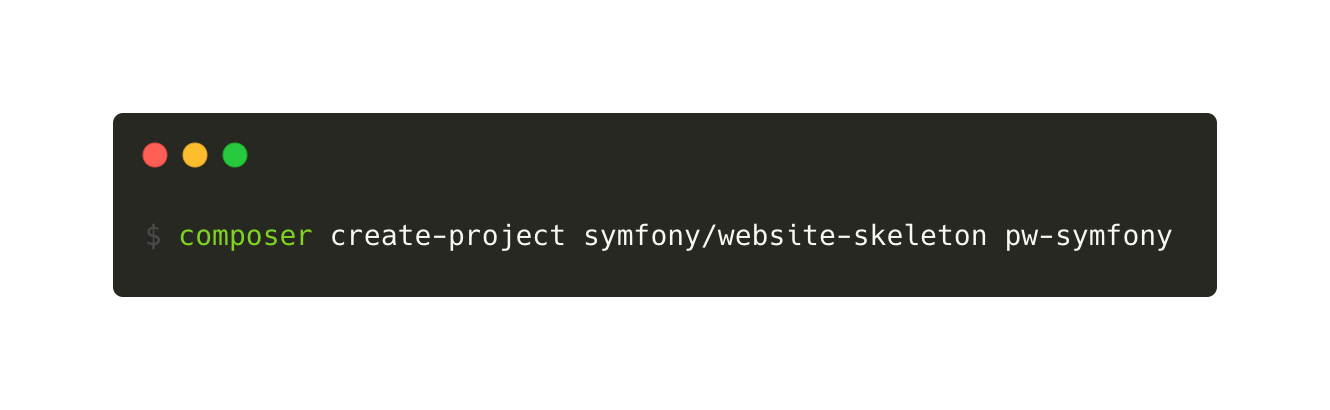
\includegraphics[width=\textwidth]{../assets/composer_create_project.png}
  \caption{Nuevo proyecto symfony con el cli}
  \label{fig:composer_create_project}
\end{figure}

Una vez creado el proyecto podemos utilizar el sevirdor intregrado en y utilizar el siguiente comando:

\begin{figure}[ht]
  \centering
  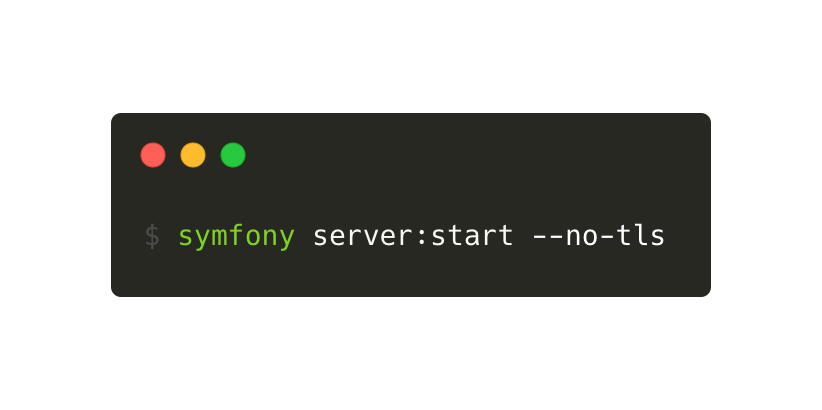
\includegraphics[width=\textwidth]{../assets/symfony_server_start.png}
  \caption{Iniciar el servidor integrado de symfony}
  \label{fig:symfony_server_start}
\end{figure}

\clearpage
Tambien podemos utilizar un servirdor apache, para que funcione bien podemos instalar el siguiente paquete:

\begin{figure}[ht]
  \centering
  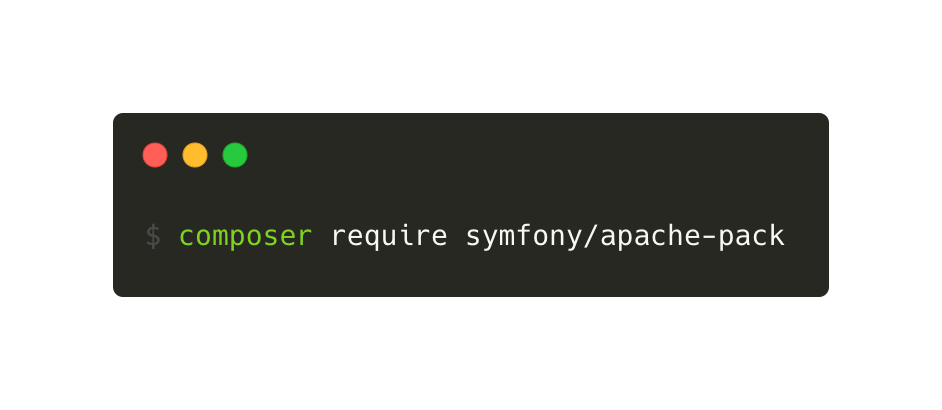
\includegraphics[width=\textwidth]{../assets/composer_apache.png}
  \caption{La forma más facil de configurar apache}
  \label{fig:composer_apache}
\end{figure}

Si todo funciona al abrir la siguiente url \href{http://localhost:8000}{http://localhost:8000} nos deberia aparecer la siguente pagina:

\begin{figure}[ht]
  \centering
  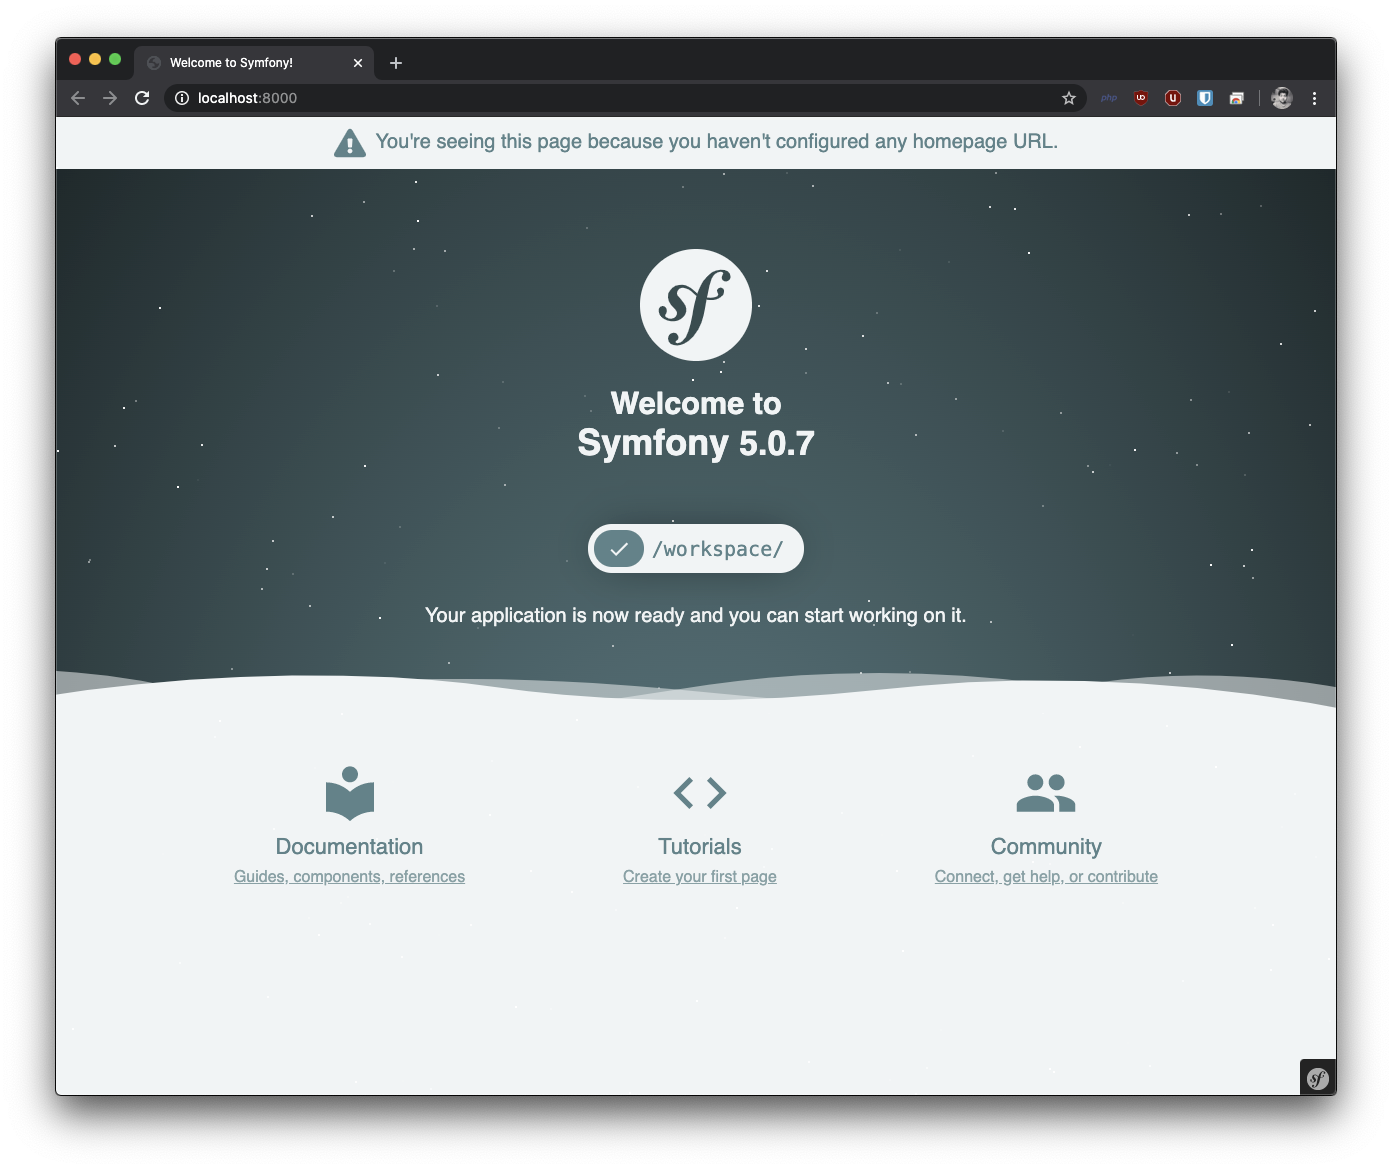
\includegraphics[width=0.7\textwidth]{../assets/symfony_main.png}
  \caption{Pagina principal symfony}
  \label{fig:symfony_main}
\end{figure}
\clearpage
\subsection{Configurando la base de datos}
Para que symfony pueda conectarse con nuestra base de datos debemos editar el fichero \texttt{.env} para modificar la varible \texttt{DATABASE\_URL}
\begin{figure}[ht]
  \centering
  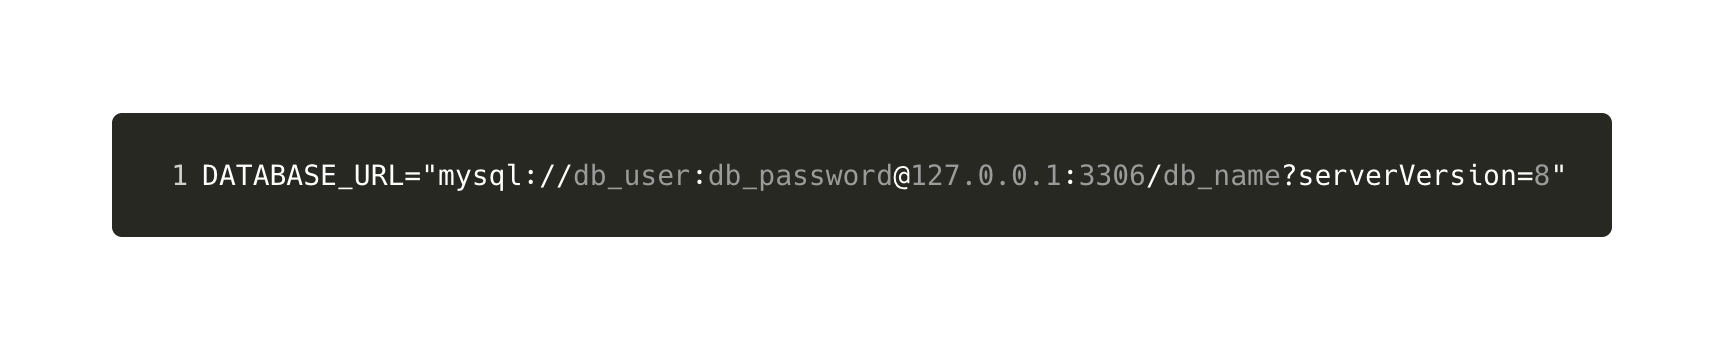
\includegraphics[width=\textwidth]{../assets/symfony_dot_env.png}
  \caption{Pagina principal symfony}
  \label{fig:symfony_dot_env}
\end{figure}

Las siguentes varible se pueden modificar acorde a nuestro caso de uso:

\begin{center}
  \begin{minipage}{0.4\textwidth}
    \begin{itemize}
      \item[mysql] Driver utilizando
      \item[db\_user] Nombre de usuario
      \item[db\_password] Contraseña del usuario
      \item[127.0.0.1] Host de la base de datos
      \item[3306] Puerto de la base de datos
      \item[serverVersion] Version de base de datos
    \end{itemize}
  \end{minipage}
\end{center}

Si antes no hemos creado nuestra base de datos podemos utilizar el siguente comando:
\begin{figure}[ht]
  \centering
  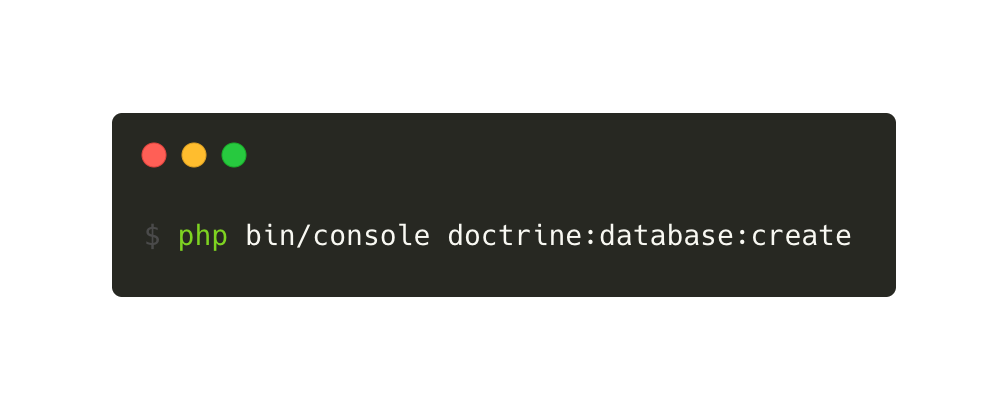
\includegraphics[width=\textwidth]{../assets/create_db.png}
  \caption{Crear base de datos}
  \label{fig:create_db}
\end{figure}
\clearpage
\subsection{Creando las Entidades}

Para crear una entididad debemos utilizar el siguiente comando:

\begin{figure}[ht]
  \centering
  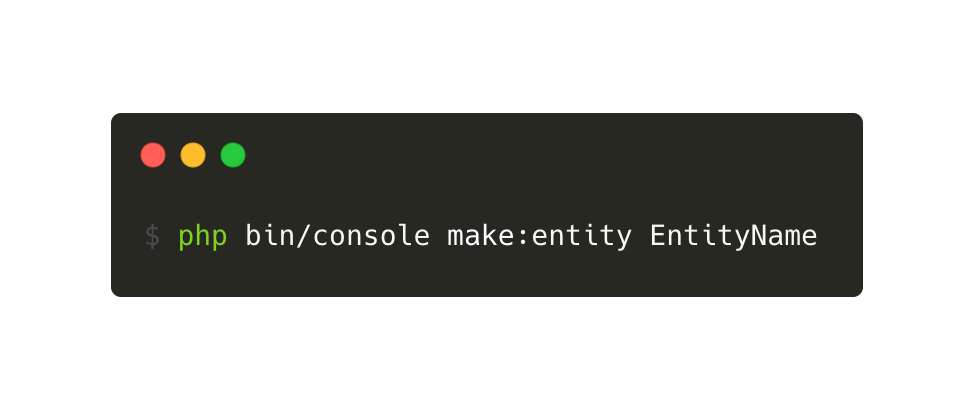
\includegraphics[width=\textwidth]{../assets/make_entity.png}
  \caption{Comando para crear una entididad}
  \label{fig:make_entity}
\end{figure}

En nuestro caso vamos a crear la entididad \texttt{Article} con las siguientes propiedades:

\begin{figure}[ht]
  \centering
  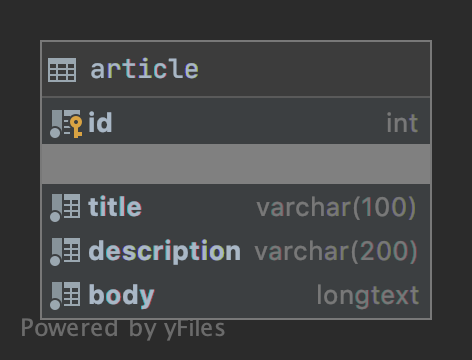
\includegraphics[width=0.4\textwidth]{../assets/article_sql.png}
  \caption{Entididad Article}
  \label{fig:article_sql}
\end{figure}

\begin{figure}[ht]
  \centering
  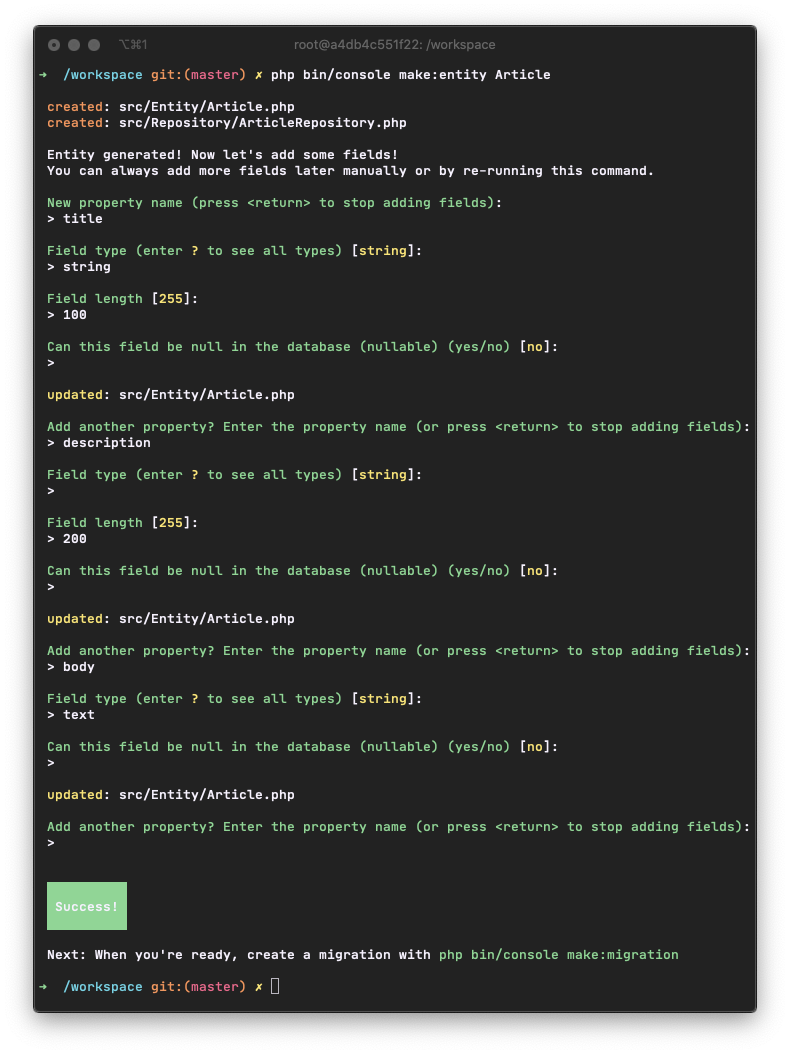
\includegraphics[width=\textwidth]{../assets/creation_article_entity.png}
  \caption{Creacion de la entidad \texttt{Article}}
  \label{fig:creation_article_entity}
\end{figure}
\clearpage

Como se puede observar en la \href{fig:creation_article_entity}{Figura anterior} el comando nos ira preguntado por la propiedades que deseamos añadir.

Una vez creada la entidad debemos hacer la migraciones ejecutando el siguiente comando:

\begin{figure}[ht]
  \centering
  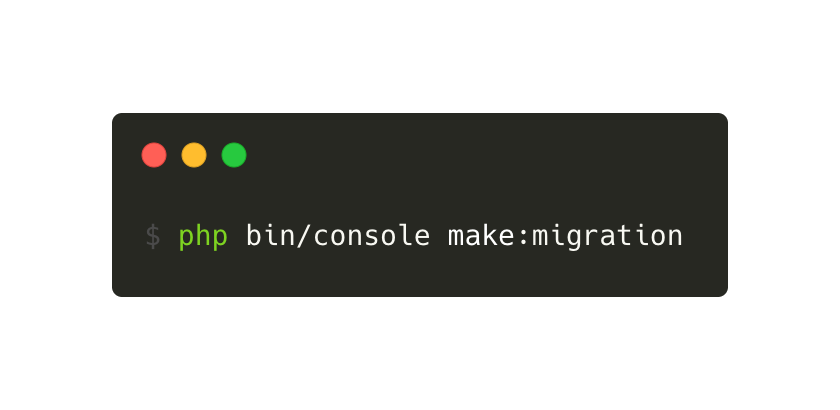
\includegraphics[width=\textwidth]{../assets/make_migration.png}
  \caption{Creando la migraciones}
  \label{fig:make_migration}
\end{figure}

Finalmente debemos aplicar la migraciones a nuestra base de datos ejecutando el siguiente comando:

\begin{figure}[ht]
  \centering
  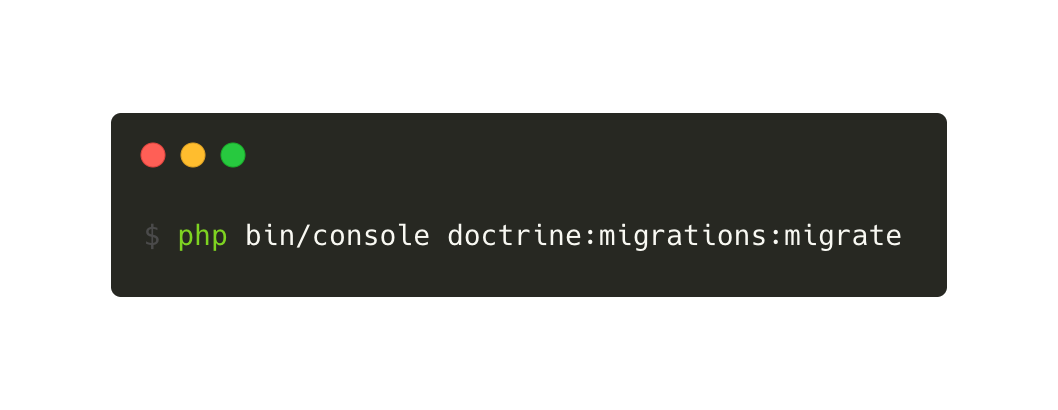
\includegraphics[width=\textwidth]{../assets/apply_migration.png}
  \caption{Aplicando las migraciones}
  \label{fig:apply_migration}
\end{figure}
\clearpage
\subsection{Creación de controlador y vistas de Artículo}

Para crear un controlador debemos utilizar el siguiente comando:

\begin{figure}[ht]
  \centering
  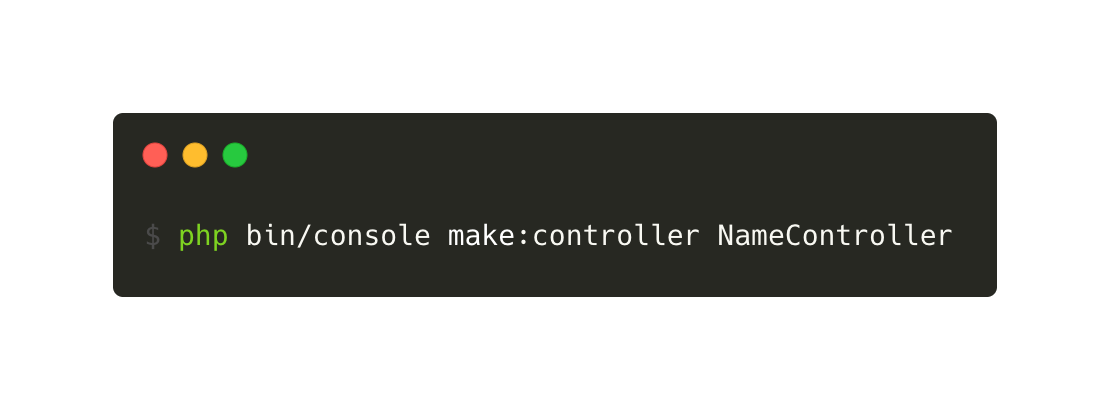
\includegraphics[width=\textwidth]{../assets/make_controller.png}
  \caption{Aplicando las migraciones}
  \label{fig:make_controller}
\end{figure}

Nos debe de crear los siguientes ficheros:


\begin{center}
  \begin{minipage}{0.4\textwidth}
    \begin{itemize}
      \item[\texttt{\textbf{src/Controller/ArticleController.php}}] Nuestro controlador.
      \item[\texttt{\textbf{templates/article/index.html.twig}}] Template por defecto.
    \end{itemize}
  \end{minipage}
\end{center}

A continuación vamos a \texttt{src/Controller/ArticleController.php}, y ahí tendremos el código de nuestro controlador de \textit{Articles}. Pasamos a dotarle de funcionalidad, como la de mostrar todos los artículos que tenemos en BD, para ello modificamos la función \texttt{index} añadiéndole lo siguiente:

\begin{figure}[ht]
  \centering
  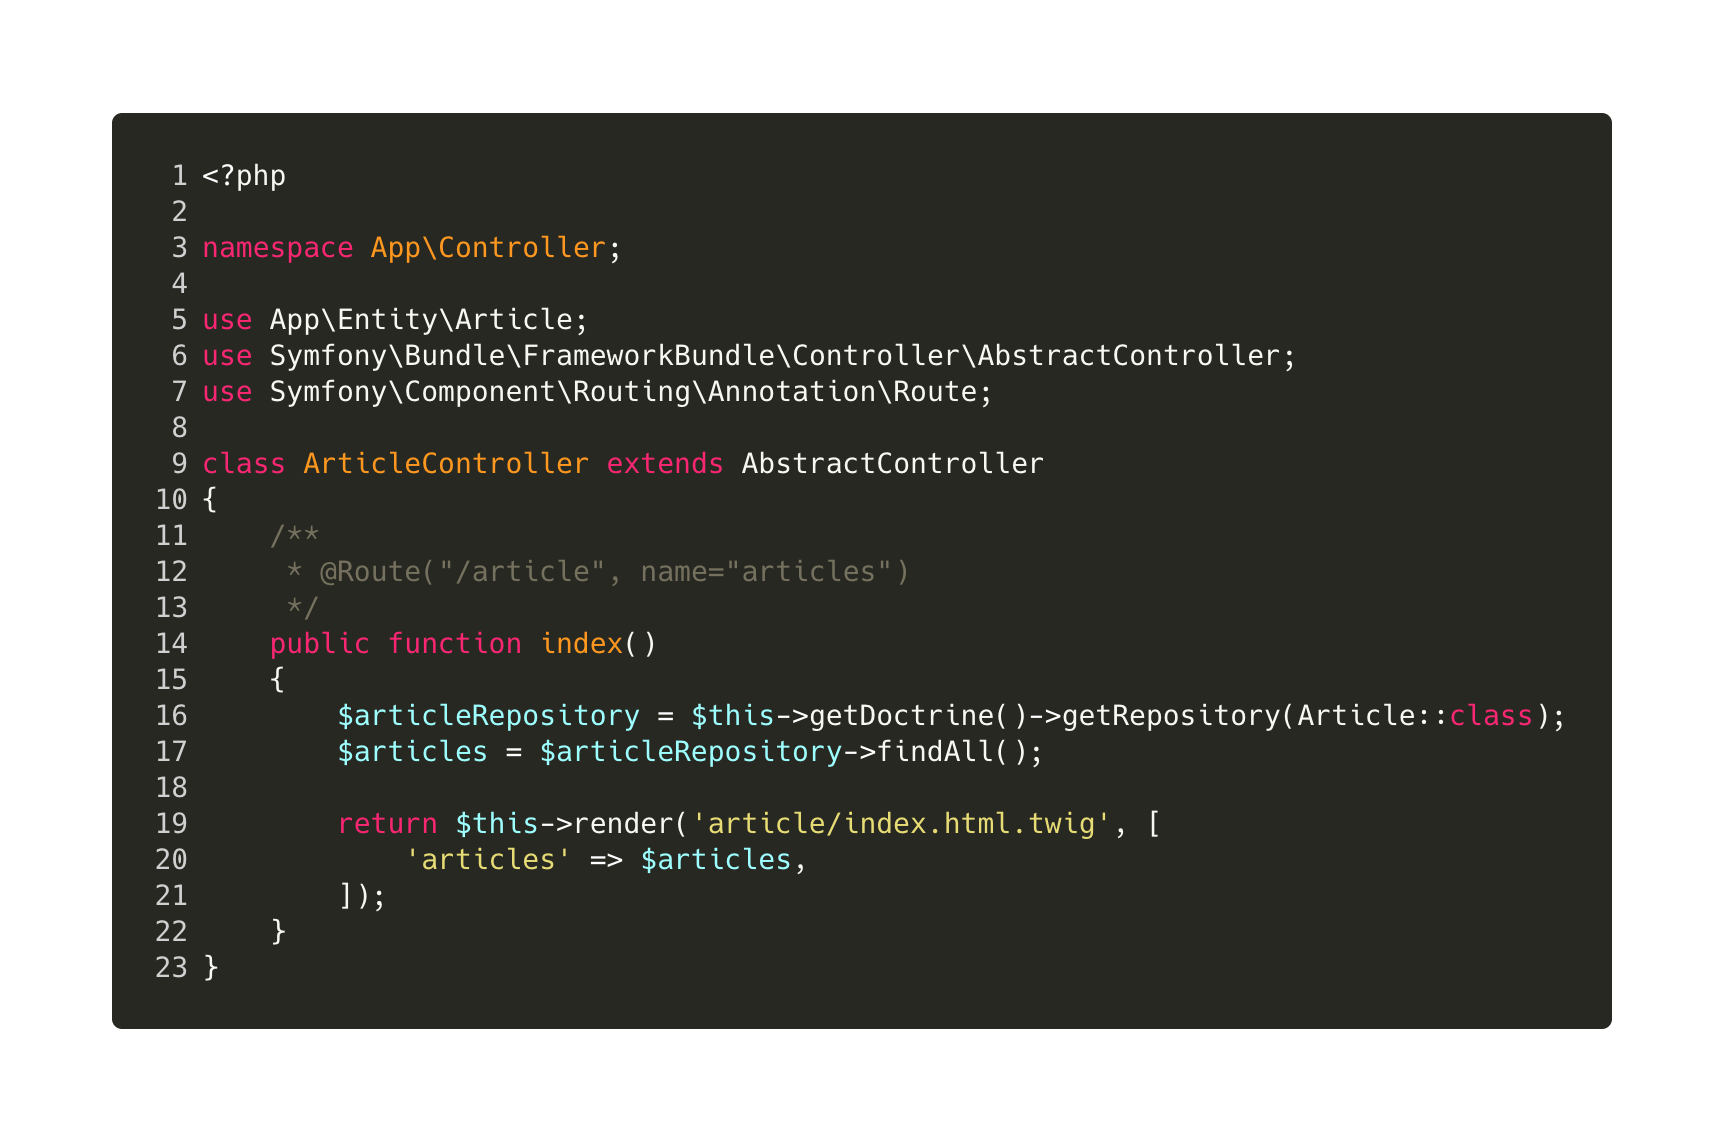
\includegraphics[width=\textwidth]{../assets/article_index.png}
  \caption{\texttt{ArticleController.php}}
  \label{fig:article_index}
\end{figure}

En la variable \texttt{\$articulosRepository} se guardará un objeto del manejador de la entidad de Doctrine, el cual es el objeto más importante en Doctrine, ya que es el responsable de guardar y obtener objetos de la base de datos.

En la variable \texttt{\$articles} se guardarán todos los artículos que se encuentren en la base de datos, y luego con el return \texttt{\$this->render()}, vamos a la vista index.\footnote{La vista plantilla ya viene creada por defecto en templates/base.html.twig y la carpeta de las vistas de Articulos también se crea sola al crear la entidad.}.

Así mismo crearemos un método llamado \texttt{show} en el controlador para mandar a una nueva vista llamada \texttt{article.html.twig} los datos de un artículo a partir de un \texttt{id}, que contendrá lo siguiente:

\begin{figure}[ht]
  \centering
  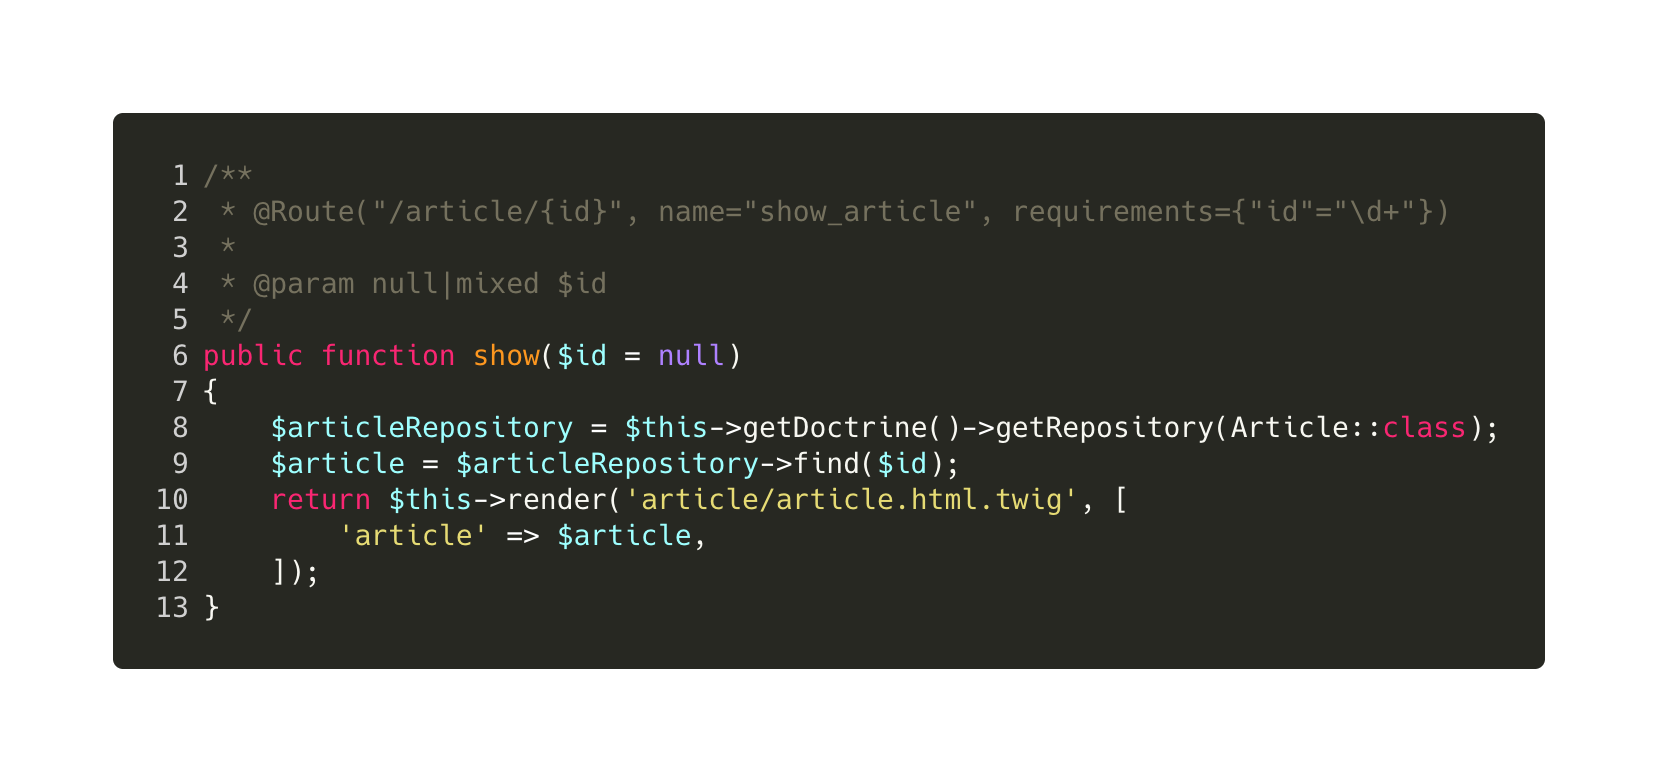
\includegraphics[width=\textwidth]{../assets/article_show.png}
  \caption{\texttt{\textbf{ArticleController::show}}}
  \label{fig:article_show}
\end{figure}

Tambien debemos editar la vista \texttt{\textbf{templates/article/index.html.twig}} con el siguente codigo:

\begin{figure}[ht]
  \centering
  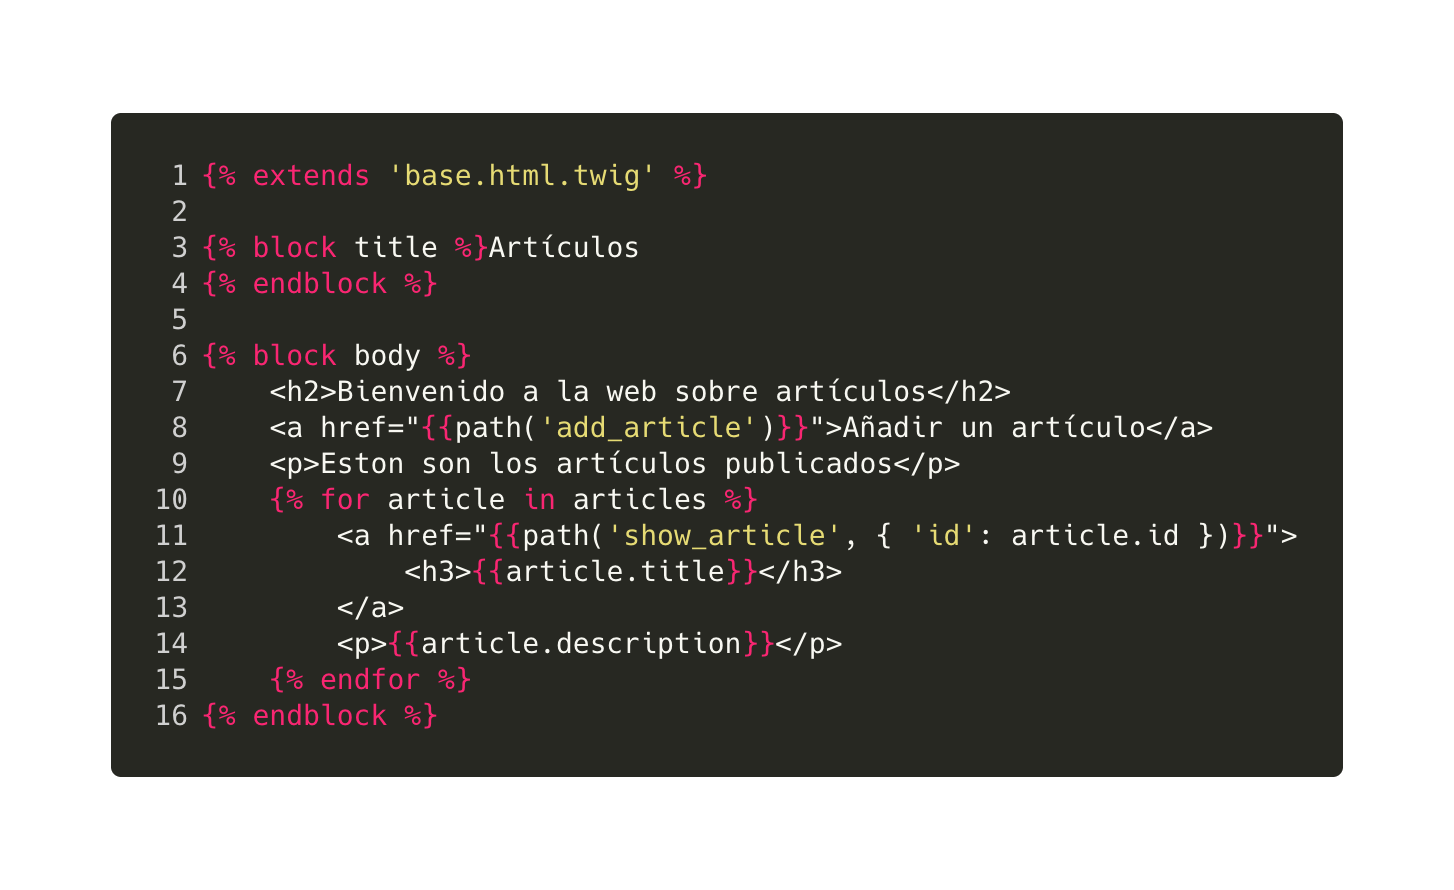
\includegraphics[width=\textwidth]{../assets/article_index_twig.png}
  \caption{Vista \texttt{\textbf{templates/article/index.html.twig}}}
  \label{fig:article_index_twig}
\end{figure}

\clearpage
Por ultimo debemos crear la vista \texttt{\textbf{templates/article/article.html.twig}} con el siguiente cotenido:

\begin{figure}[ht]
  \centering
  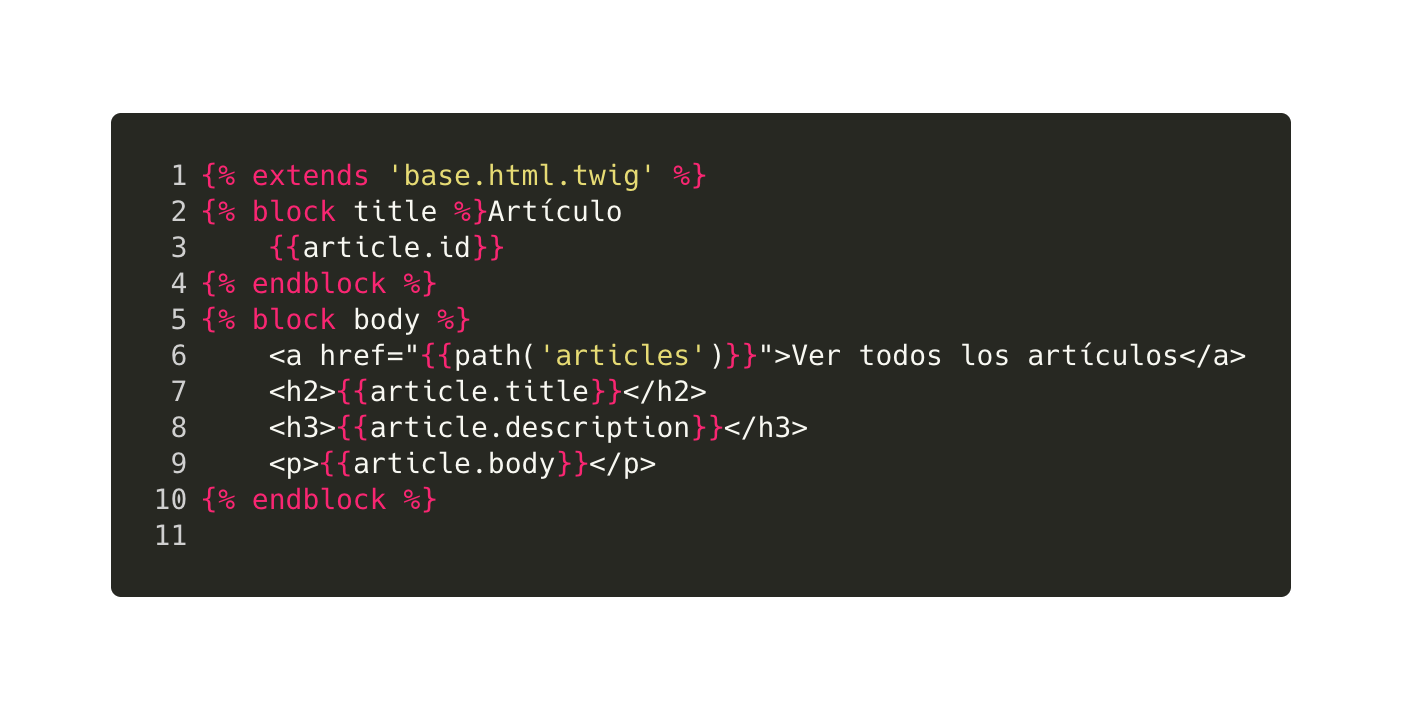
\includegraphics[width=\textwidth]{../assets/article_article.png}
  \caption{Vista \texttt{\textbf{templates/article/article.html.twig}}}
  \label{fig:article_article}
\end{figure}

\subsection{Creación de Formularios}

Para crear un formulario utilizaremos el siguiente comando:

\begin{figure}[ht]
  \centering
  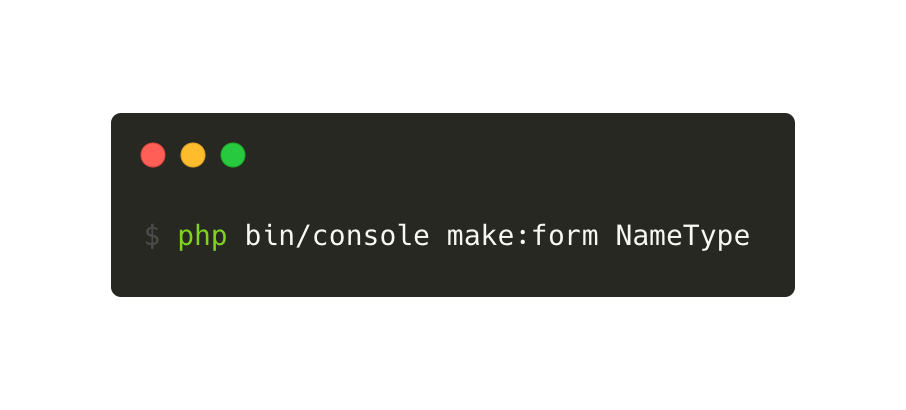
\includegraphics[width=\textwidth]{../assets/make_form.png}
  \caption{Comando para crear un formulario}
  \label{fig:make_form}
\end{figure}

\clearpage
Este comando nos generara el fichero \texttt{\textbf{src/Form/ArticleType.php}}, al que debemos editar con el siguiente código:

\begin{figure}[ht]
  \centering
  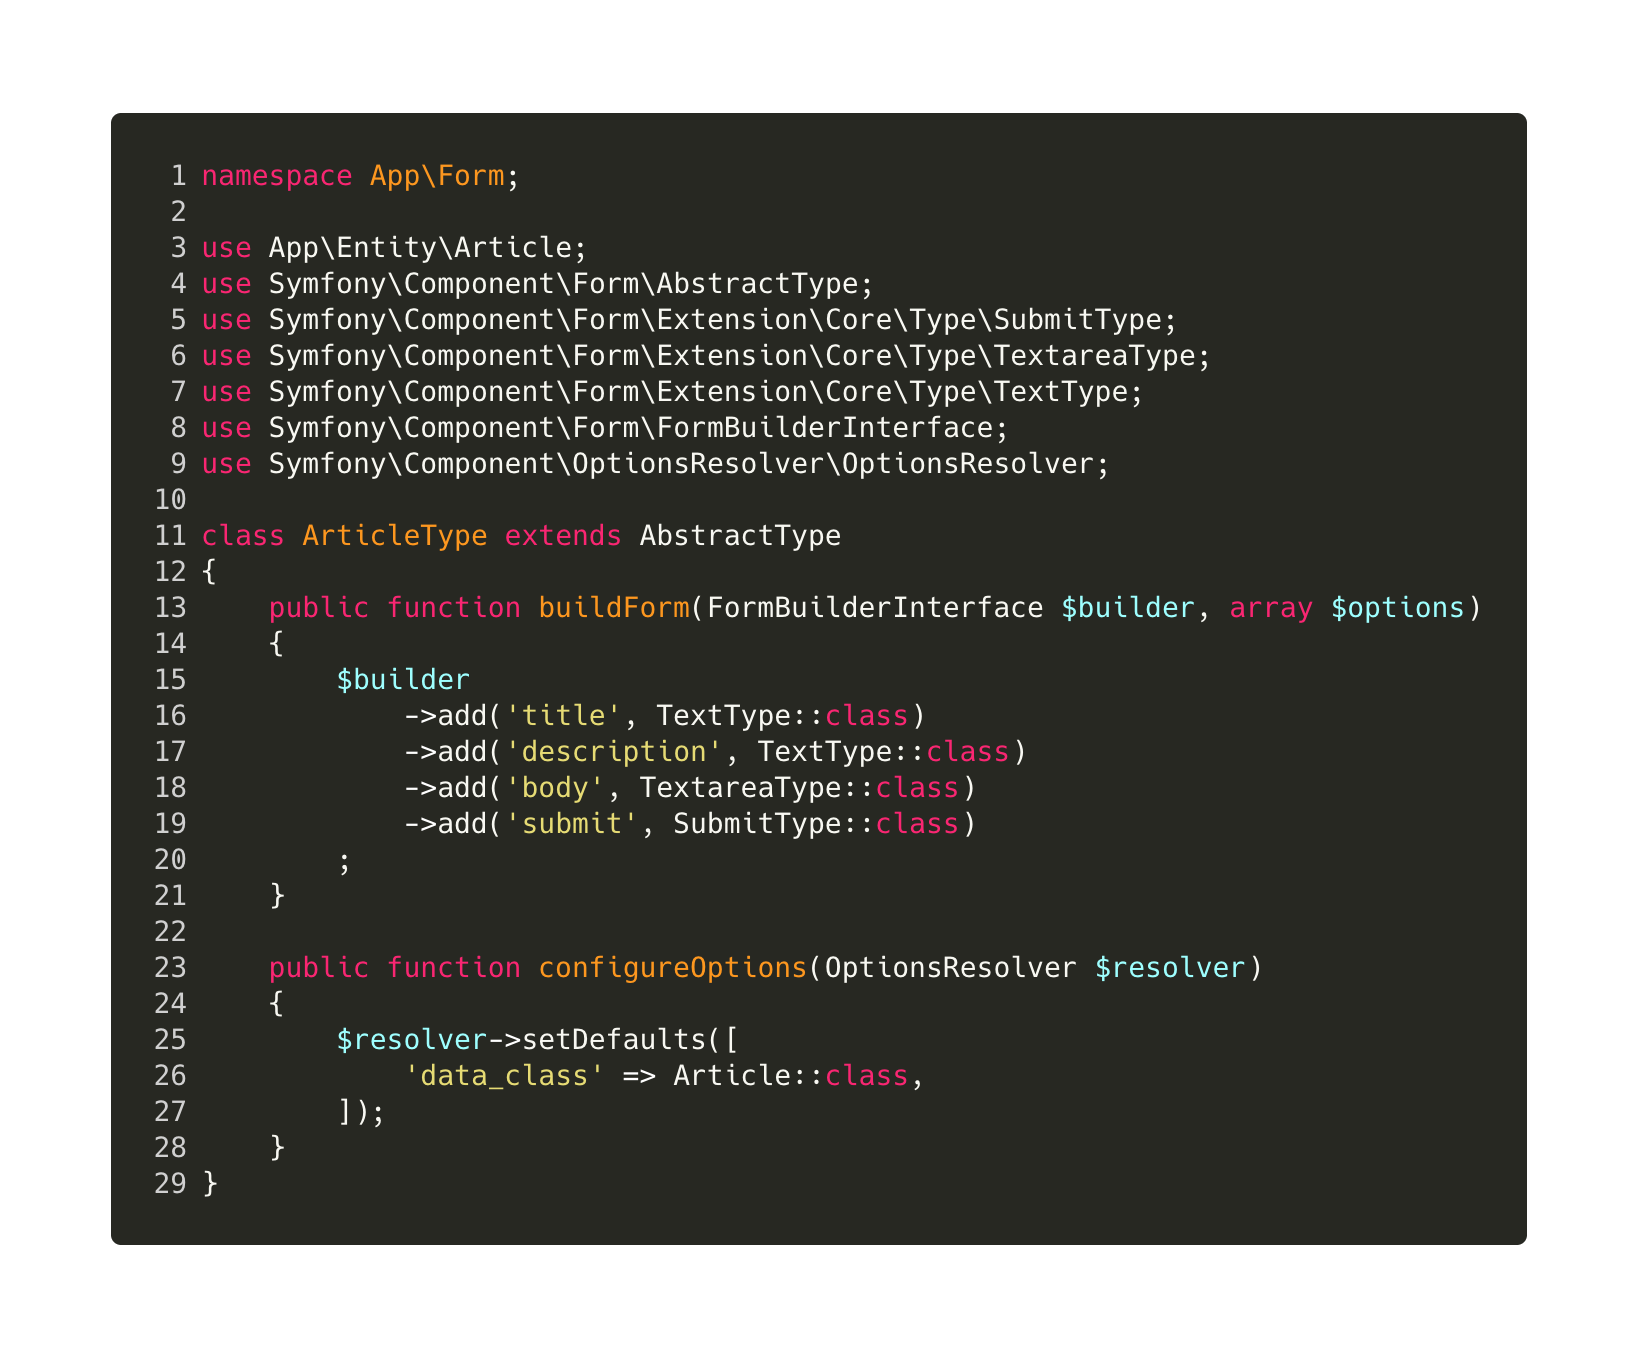
\includegraphics[width=\textwidth]{../assets/article_type.png}
  \caption{\texttt{\textbf{ArticleType}}}
  \label{fig:article_type}
\end{figure}

Después de haber creado el formulario, pasamos a crear la función de crear un nuevo artículo, y su vista correspondiente.
\clearpage
A la función la llamaremos \texttt{create}, su código será el siguiente:
\begin{figure}[ht]
  \centering
  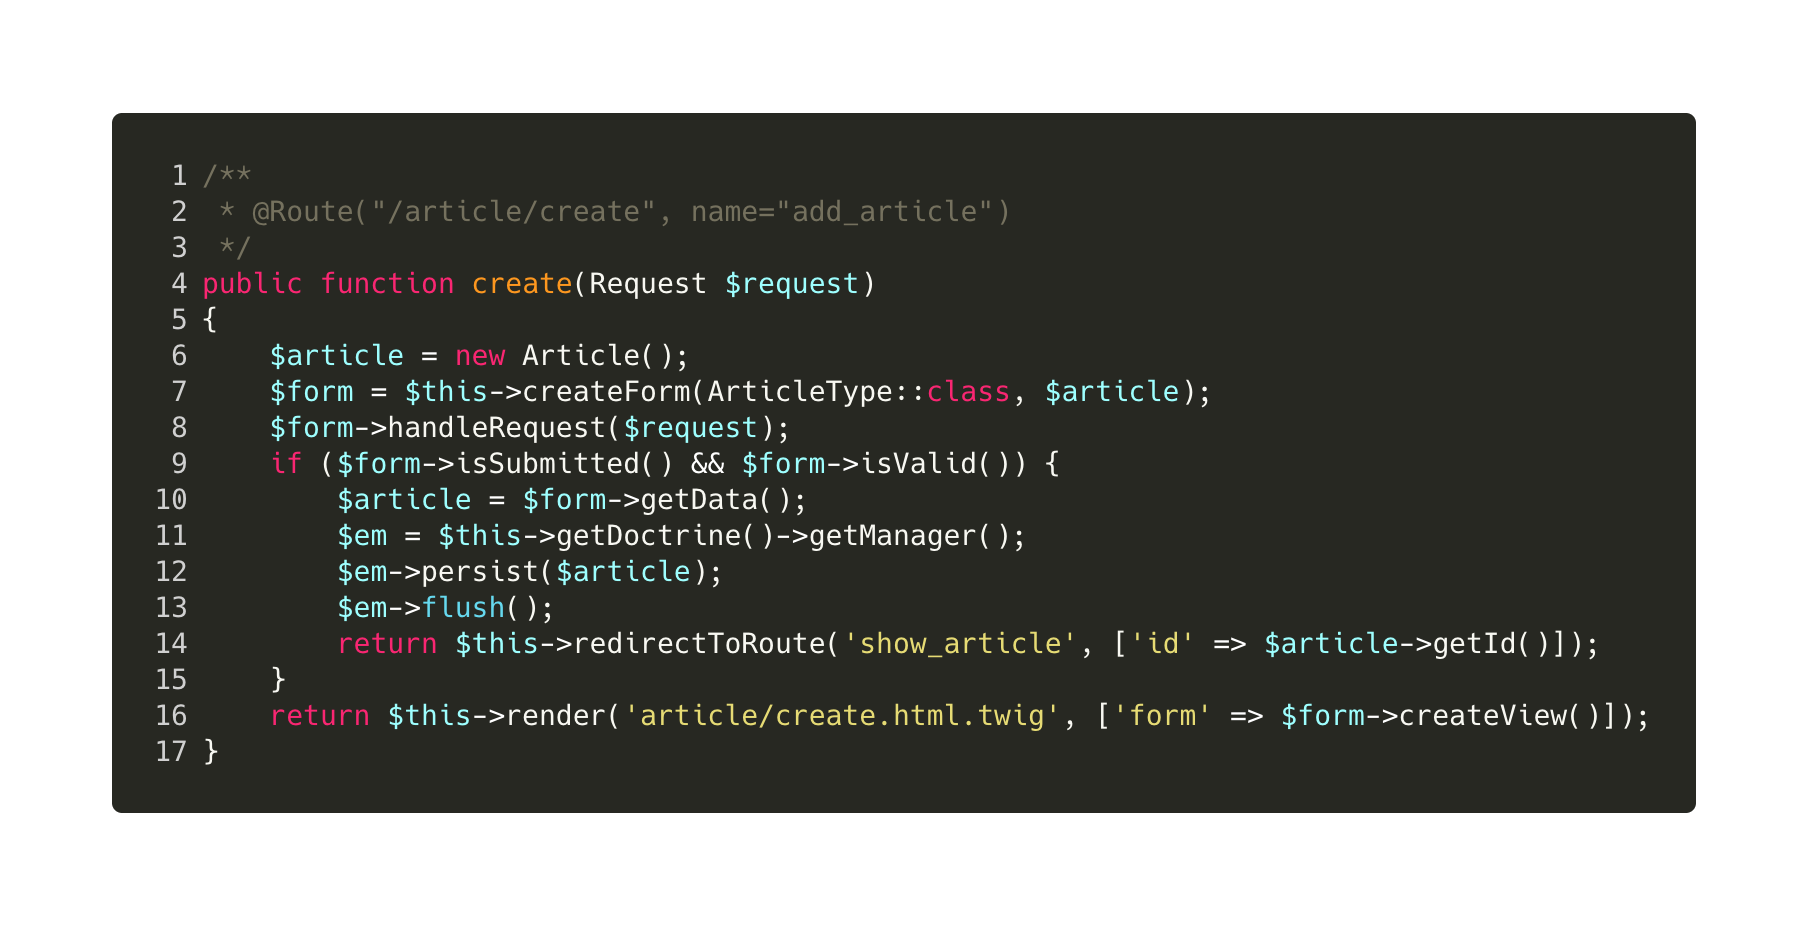
\includegraphics[width=\textwidth]{../assets/article_create_form.png}
  \caption{\texttt{\textbf{ArticleController::create}}}
  \label{fig:article_create_form}
\end{figure}

El codigo de la vista \texttt{\textbf{templates/article/create.html.twig}} es el siguente:

\begin{figure}[ht]
  \centering
  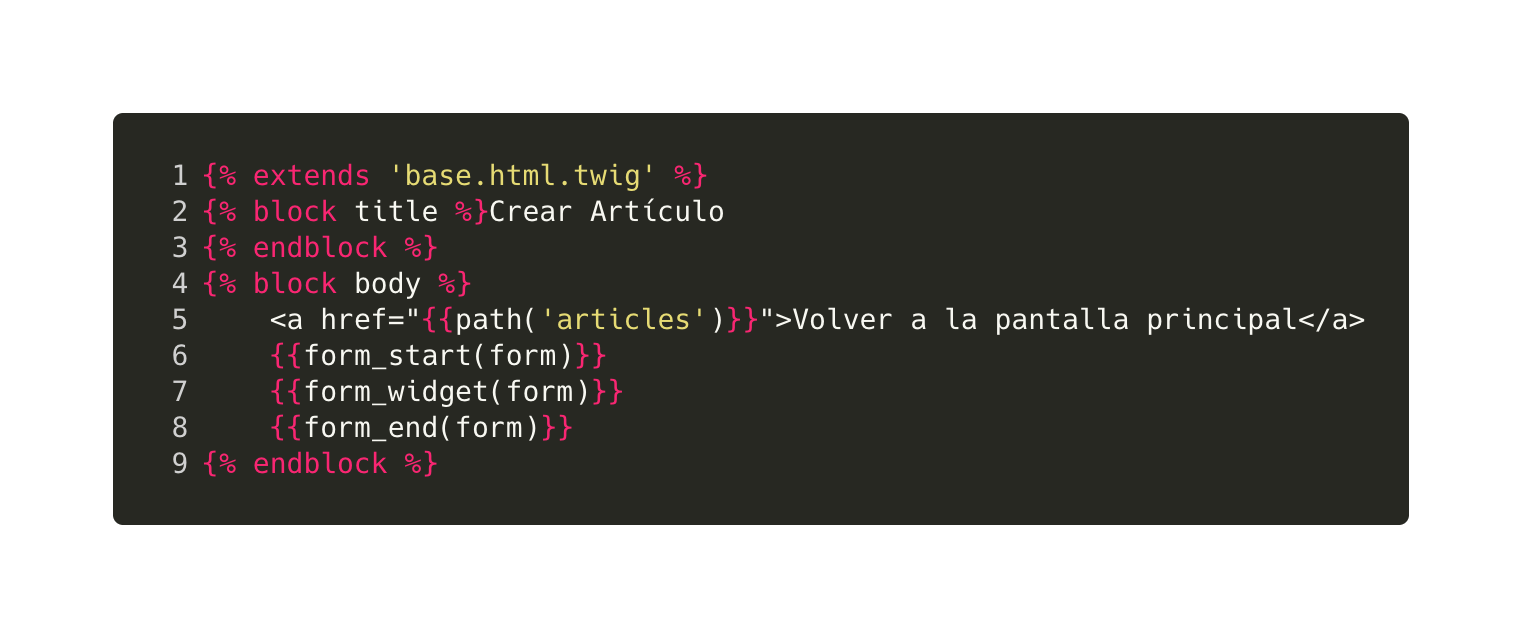
\includegraphics[width=\textwidth]{../assets/form_article_twig.png}
  \caption{Vista \texttt{\textbf{templates/article/create.html.twig}}}
  \label{fig:form_article_twig}
\end{figure}

\clearpage
Ahora si vamos a \texttt{http://localhost:8888/article} veremos la siguente vista:

\begin{figure}[ht]
  \centering
  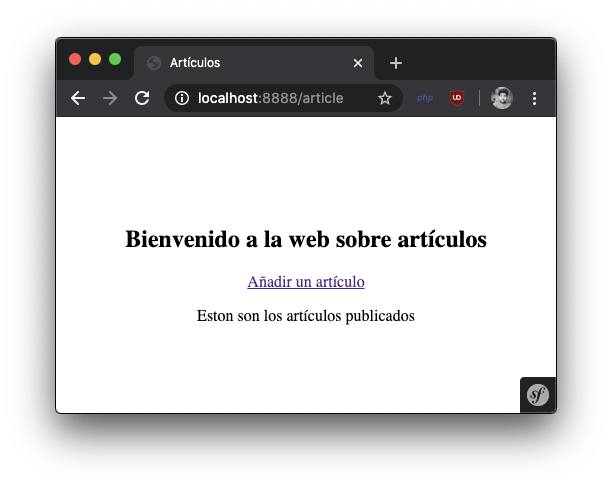
\includegraphics[width=\textwidth]{../assets/articles_render.png}
  \caption{Ruta \texttt{\textbf{article}}}
  \label{fig:articles_render}
\end{figure}

\clearpage
Si le damos a \textit{Añadir un artículo}, nos mandará la vista del \href{fig:article_create_form}{formulario} que hemos creado para crear nuestros artículos.

\begin{figure}[ht]
  \centering
  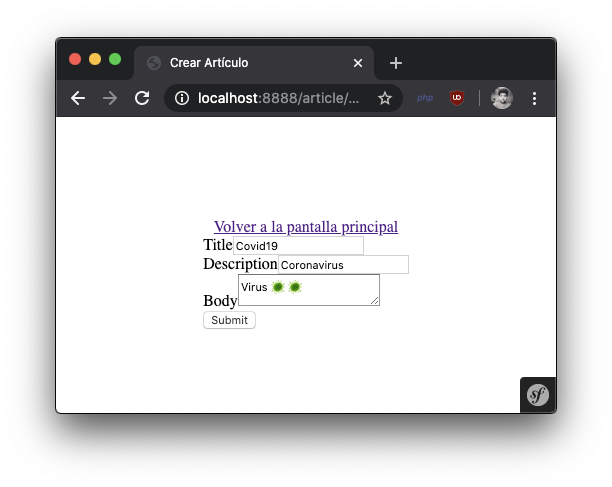
\includegraphics[width=\textwidth]{../assets/article_form_render.png}
  \caption{Ruta \texttt{\textbf{article/create}}}
  \label{fig:article_form_render}
\end{figure}

\clearpage
Para probar que funciona añadiremos los datos de un artículo de ejemplo y veremos que al hacer \texttt{submit} nos mandará a la vista de este artículo en concreto.

\begin{figure}[ht]
  \centering
  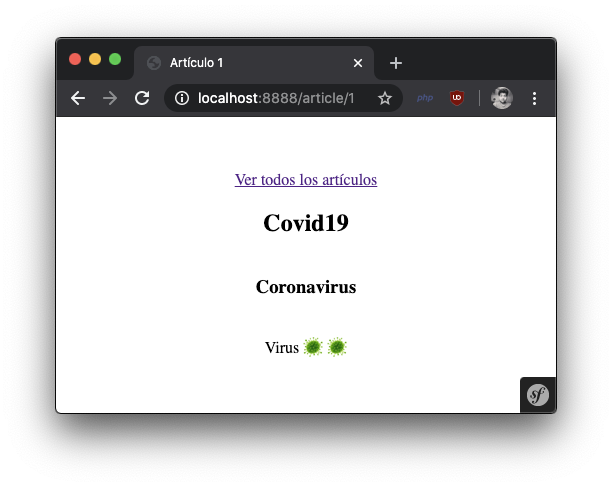
\includegraphics[width=\textwidth]{../assets/article_render.png}
  \caption{Ruta \texttt{\textbf{article/1}}}
  \label{fig:article_render}
\end{figure}


\clearpage
\nocite{*}
\printbibliography

\end{document}
